% !TeX root = Thesis.tex
% !TeX spellcheck = en_GB
% Copyright (C) 2014-2016 by Thomas Auzinger <thomas@auzinger.name>

\documentclass[
%draft,
final,
%headings=openany
]{vutinfth} % Remove option 'final' to obtain debug information.

% Load packages to allow in- and output of non-ASCII characters.
\usepackage{lmodern}        % Use an extension of the original Computer Modern font to minimize the use of bitmapped letters.
\usepackage[T1]{fontenc}    % Determines font encoding of the output. Font packages have to be included before this line.
\usepackage[utf8]{inputenc} % Determines encoding of the input. All input files have to use UTF8 encoding.

% Extended LaTeX functionality is enables by including packages with \usepackage{...}.
%\usepackage{fixltx2e}   % Provides fixes for several errors in LaTeX2e.
\usepackage{amsmath}    % Extended typesetting of mathematical expression.
\usepackage{amssymb}    % Provides a multitude of mathematical symbols.
\usepackage{mathtools}  % Further extensions of mathematical typesetting.
\usepackage{microtype}  % Small-scale typographic enhancements.
\usepackage{enumitem}   % User control over the layout of lists (itemize, enumerate, description).
\usepackage{multirow}   % Allows table elements to span several rows.
\usepackage{booktabs}   % Improves the typesettings of tables.
\usepackage{subcaption} % Allows the use of subfigures and enables their referencing.
\usepackage[ruled,linesnumbered,algochapter]{algorithm2e} % Enables the writing of pseudo code.
\usepackage[usenames,dvipsnames,table]{xcolor} % Allows the definition and use of colors. This package has to be included before tikz.
\usepackage{nag}       % Issues warnings when best practices in writing LaTeX documents are violated.
\usepackage{todonotes} % Provides tooltip-like todo notes.
\usepackage[autostyle]{csquotes}
\usepackage{hyperref}  % Enables cross linking in the electronic document version. This package has to be included second to last.
\usepackage[acronym,toc]{glossaries} % Enables the generation of glossaries and lists fo acronyms. This package has to be included last.

% Define convenience functions to use the author name and the thesis title in the PDF document properties.
\newcommand{\authorname}{Martin Weik} % The author name without titles.
\newcommand{\thesistitle}{REAc based IFRS Accrual Accounting} % The title of the thesis. The English version should be used, if it exists.
\newcommand{\thesissubtitle}{Modeling IFRS accrual accounting based on the REAc accounting model}

% Set PDF document properties
\hypersetup{
    pdfpagelayout   = TwoPageRight,           % How the document is shown in PDF viewers (optional).
    linkbordercolor = {Melon},                % The color of the borders of boxes around crosslinks (optional).
    pdfauthor       = {\authorname},          % The author's name in the document properties (optional).
    pdftitle        = {\thesistitle},         % The document's title in the document properties (optional).
    pdfsubject      = {Subject},              % The document's subject in the document properties (optional).
    pdfkeywords     = {a, list, of, keywords} % The document's keywords in the document properties (optional).
}

\setsecnumdepth{subsection} % Enumerate subsections.
\setlist{nolistsep} % Spacing before and after lists

\nonzeroparskip             % Create space between paragraphs (optional).
\setlength{\parindent}{0pt} % Remove paragraph identation (optional).

% \makeindex      % Use an optional index.
% \makeglossaries % Use an optional glossary.
% \glstocfalse   % Remove the glossaries from the
% table of contents.

% Set persons with 4 arguments:
%  {title before name}{name}{title after name}{gender}
%  where both titles are optional (i.e. can be given as empty brackets {}).
\setauthor{}{\authorname}{BSc}{male}
\setadvisor{Univ.Prof. Mag.rer.soc.oec. Dr.rer.soc.oec.}{Walter Schwaiger}{}{male}
%\setaddress{Adresse anpassen!}

% For bachelor and master theses:
%\setfirstassistant{Pretitle}{Forename Surname}{Posttitle}{male}
%\setsecondassistant{Pretitle}{Forename Surname}{Posttitle}{male}
%\setthirdassistant{Pretitle}{Forename Surname}{Posttitle}{male}

% For dissertations:
%\setfirstreviewer{Pretitle}{Forename Surname}{Posttitle}{male}
%\setsecondreviewer{Pretitle}{Forename Surname}{Posttitle}{male}

% For dissertations at the PhD School:
%\setsecondadvisor{Pretitle}{Forename Surname}{Posttitle}{male}

% Required data.
\setregnumber{00026006 Stand \today}
\setdate{12}{11}{2023} % Set date with 3 arguments: {day}{month}{year}.

\settitle{\thesistitle}{\thesistitle} % Sets English and German version of the title (both can be English or German).
\setsubtitle{\thesissubtitle}{\thesissubtitle} % Sets English and German version of the subtitle (both can be English or German).

% Select the thesis type: bachelor / master / doctor / phd-school.
% Bachelor:
%\setthesis{bachelor}
%
% Master:
\setthesis{master}
\setmasterdegree{dipl.} % dipl. / rer.nat. / rer.soc.oec. / master

%
% Doctor:
%\setthesis{doctor}
%\setdoctordegree{rer.soc.oec.}% rer.nat. / techn. / rer.soc.oec.
%
% Doctor at the PhD School
%\setthesis{phd-school} % Deactivate non-English title pages (see below)

% For bachelor and master:
\setcurriculum{Business Informatics}{Wirtschaftsinformatik} % Sets the English and German name of the curriculum.

% For dissertations at the PhD School:
%\setfirstreviewerdata{Affiliation, Country}
%\setsecondreviewerdata{Affiliation, Country}

% Define convenience macros.
%\newcommand{\todo}[1]{{\color{red}\textbf{TODO: {#1}}}} % Comment for the final version, to raise errors.



\begin{document}
\frontmatter % Switches to roman numbering.
% The structure of the thesis has to conform to
%  http://www.informatik.tuwien.ac.at/dekanat

\addtitlepage{naustrian} % German title page (not for dissertations at the PhD School).
\addtitlepage{english} % English title page.
\addstatementpage

%\begin{danksagung*}
%	\todo{Ihr Text hier.}
%\end{danksagung*}
%
%\begin{acknowledgements*}
%	\todo{Enter your text here.}
%\end{acknowledgements*}
%
%\begin{kurzfassung}
%	\todo{Ihr Text hier.}
%\end{kurzfassung}
%
%\begin{abstract}
%	\todo{Enter your text here.}
%\end{abstract}


% Select the language of the thesis, e.g., english or naustrian.
\selectlanguage{english}

% Add a table of contents (toc).
\tableofcontents % Starred version, i.e., \tableofcontents*, removes the self-entry.


% Switch to arabic numbering and start the enumeration of chapters in the table of content.
\mainmatter

%this controls the width of long captions
\captionsetup{width=0.8\textwidth}

% !TeX spellcheck = en_GB
% !TEX root = Thesis
\chapter{Introduction}\label{chap01}
%\begin{itemize}
%	\item REA in short (like Schwaiger
%	\item motivating example: ELMO basis -> Accrual accounting, is a transition possible?, How does it look like?, Elements even in basic accrual accounting: equity, tax, are they missing? how can rea be enhanced?
%	\item Application in IFRS: complete information
%	\item Table
%\end{itemize}

\section{Ressources, Events, Agents}\label{sec:REAIntroduction}

McCarthy introduced REA with accountants and double-entry bookings in mind: “...time to rethink some of the basic constructs of traditional double-entry bookkeeping.” \cite{mccarthy1982rea}, p.554.
It definitely has it's mares by introducing quantities and connecting events that belong to one business transaction.

Very important elements for accrual accounting like liabilities, deprecations are mentioned but not fully conceptualized.
The basic model is focusing on realised events and therefore can only handle tangible \& intangible assets and cash as resources that can be traded on a spot-market.

Elements beyond spot-market are discussed as discrepancies between the view of accountants and non-accountants, e.g. on accruals:
"Cases where they probably would disagree would involve accruals such as wage expense or interest revenue." \cite{mccarthy1982rea}, p. 572.
Even if issues are identified, only different approaches are considered without any final verdict.

\section{Motivating example}\label{sec:motivation}
Figure \ref{fig:rea-initial-example-taken-from-bill-mccarthys-presentation} take from MaCarty's introduction into REA \cite{mccarthy2004elmo-cookie-monster} visualizes a very basic example of a REA instance where the Cookiemonster buys cookies from ELMO and pays in cash.
In fact two events happen at the same time: There is a sales event happening handing over cookies from ELMO to the cookiemonster and at the same time the cash receipt is happening where cookiemonster pays for the received cookies.
The whole diagram visualizes this exchanges of money for cookies and the duality between give and take.

\begin{figure}
	\centering
	\caption{REA Initial Example}
	\label{fig:rea-initial-example-taken-from-bill-mccarthys-presentation}
	\includegraphics[width=0.7\linewidth]{"../figures/REA Initial Example taken from Bill McCarthy's Presentation"}
	\caption*{This figure is taken from Bill McCarthy's Presentation\cite{mccarthy2004elmo-cookie-monster} shows and shows the exchange of cookies against money betwen Elmo and the Cookimonster.}
\end{figure}

\begin{table}
	\caption{Strongly Simplified balance sheet at beginning of period}\label{tab:intro:accrual1}
	
	\begin{subtable}{.5\linewidth}
		\centering
		\caption{Assets}
		\begin{tabular}{|c|c|}
			\hline
			Account & Amount \\ 
			\hline 
			Stocks & 1.000,- \\ 
			\hline
		\end{tabular}
	\end{subtable}
	\begin{subtable}{.5\linewidth}
		\centering
		\caption{Liabilities}
		\begin{tabular}{|c|c|}
			\hline
			Account & Amount \\ 
			\hline 
			Equity & 1.000,- \\ 
			\hline
		\end{tabular}
	\end{subtable}
	\bigskip
	\caption{P\&L accounts of the transaction}\label{tab:intro:accrual2}
	\begin{center}
		\begin{tabular}{|c|c|c|c|}
			\hline 
			Account & Account Type & Debit Amount & Credit Amount \\ 
			\hline 
			Cash & Asset & 200,- & \\
			\hline
			Sales of goods & P\&L & & 160,- \\ 
			\hline
			Pre-tax (VAT) & Liability & & 40,- \\
			\hline 
			Stocks & Assets & & 130,- \\
			\hline 
			Cost of sales & P\&L & 130,- & \\
			\hline
		\end{tabular}
	\end{center}
	\bigskip
	\caption{Strongly Simplified balance sheet after transaction}\label{tab:intro:accrual3}
	\begin{subtable}{.5\linewidth}
		\centering
		\caption{Assets}
		\begin{tabular}{|c|c|}
			\hline
			Account & Amount \\
			\hline
			Cash & 200 \\
			\hline 
			Stocks & 870,- \\ 
			\hline
		\end{tabular}
	\end{subtable}
	\begin{subtable}{.5\linewidth}
		\centering
		\caption{Liabilities}
		\begin{tabular}{|c|c|}
			\hline
			Account & Amount \\ 
			\hline 
			Equity & 1.030,- \\ 
			\hline
			Pre-Tax & 40,- \\ 
			\hline
		\end{tabular}
	\end{subtable}
\end{table}


Tables \ref{tab:intro:accrual1}, \ref{tab:intro:accrual2} and \ref{tab:intro:accrual3} show in a simplified manner the corresponding artefacts in accrual accounting, 
\ref{tab:intro:accrual1} the initial balance sheet, 2) the double-entry bookings in an accounting system and 3) the resulting balance sheet.
The sales event can be mapped to cost of sales, as inventory is lowering stocks:
It implies a "loss" and is therefore an event that leads to a booking on the credit side of an P\&L account whereas the cash receipt event can be mapped to turnover in P\&L on debit side as cash raises the cash in hand account.

\enquote{Debit} and \enquote{Credit} are terms commonly used in \enquote{Double Entry Accounting} \todo{Fertigstellen oder bleiben lassen} jj


The VAT visible in table \ref{tab:intro:accrual2} is typical for the mentioned misalignment between accountants and non-accountants\cite{mccarthy1982rea}, p. 572:
From a pure business process view it is irrelevant as it has no effect on the activities of the business unit.
But a company cannot neglect the obligation to collect VAT from end-customers and forward it to the tax authority.

So to support the initial idea of \enquote{A Generalized Framework for Accounting Systems in a Shared Data Environment} \cite{mccarthy1982rea}, it is necessary to reflect not the business view alone but also the accountant view.
This thesis main subject will be to identify semantic counterparts in both REA and accrual accounting if not yet defined and to define an interpretation of REA models into the view of accrual accounting.
\section{Possible positive aspects of REA for accrual accounting}
REA was inventend for general accounting in a shared memory environment.

IFRS principles say that the balance sheet has to give a detailed view.\todo{Write about positive effects}

Example: Debts often have a due date included, this has to be followed up in a separate list outside of double entry accounting. With the possibilities of REA (including policies) all informations: values, agents and due dates can be stored in the same place.

\section{Problem statement - Analysis of REA in context of accrual accounting}

Table \ref{tab:accrualaccounting} compares important elements of accrual accounting with the REA accounting model and shows where further investigations are needed.
This task is done in chapters \ref{chap:REA} and \ref{chap:accounting}.\todo{Überarbeiten}

%how elements of accrual accounting can be mapped already and where further investigation is needed.
%Definitions beyond spot-market elements are vague and 
So it's especially unclear how important statements for accrual accounting can be generated out of a REA based model:
\begin{itemize}[noitemsep]%,topsep=0pt,parsep=0pt,partopsep=0pt]
	\item Balance sheet
	\item Profit \& loss
	\item Cash flow analysis
	\item Changes in equity
\end{itemize}
Although REA evolved more and more to a inter-company modelling language it has still good properties for modelling accrual accounting also.
Target of this thesis is therefore to conceptualize a REA-based accrual accounting model and to show that it covers all key element for accrual accounting.
\begin{table}
	\caption{Accrual accounting and REA Accounting Model comparison}\label{tab:accrualaccounting}
\begin{center}
\begin{tabular}{|p{3,5cm}|p{5,8cm}|p{5,8cm}|}
	\hline 
	Accrual accounting & REA Accounting Model \cite{mccarthy1982rea} & Shortcomings \\ 
	\hline 
	Assets (A) & Tangible and intangible assets are modelled as resources. Receivables are not explicitly covered in the original model; proposed is a claim as “imbalanced” REA model on pages 567f. %\cite{mccarthy1982rea}
%	Later commitments are introduced to model them as future exchange of resources \cite{mccarthy2006reapolicy}
	& An investigation for each type of receivable is needed, if existing elements in REA are sufficient (e.g. ageing). \\ 
	\hline 
	Liabilities (L) & Liabilities are not explicitly covered in the original model; proposed is a claim as “imbalananced” REA model on pages 567f. %\cite{mccarthy1982rea}
%	Later commitments are introduced to model them as future exchange of resources \cite{mccarthy2006reapolicy}
	& An investigation for each type of liability is needed, if existing elements in REA are sufficient (e.g. ageing). \\ 
	\hline 
	Equity (E) & %\cite{mccarthy1982rea} 
	Equity is defined as residual size. It is proposed to identify “equity investments” and “dividend distribution” as explicit events to model the structure of equity on page 575. & This approach leaves out the definition of equity via the changes-in-equity statement which is a very important artifact in accrual accounting. \\
	\hline
	P\&L accounts (E) & %In \cite{mccarthy1982rea}
	 P\&L accounts are mapped to Events. & As events are realisations, future events and connected resource flows need to be discussed. \\ 
	\hline 
	Depreciations (E \& A) & On page 574 modelling as “related” connections via “macro-level duality” links to multiple corresponding materialized events is proposed. & As depreciations are usually loosely coupled to specific events a more generic approach is needed. \\ 
	\hline
	Provisions (E \& L)  & Provisions are not explicitly covered in \cite{mccarthy1982rea}. & As provisions are future events with a certain probability without underlying contract it's not yet defined how to model them with existing elements of the REA accounting model. \\
	\hline
%	stock revaluation
%	& under deprecation?? &
%	\\
%	\hline
	Accruals ( A or E \& L ) & These are mentioned as “approximate partitions of exchange transactions” on  page 572 and no definite conclusion is done. & In accrual accounting it is sometimes necessary to recognize expenses before the related exchange event has happened. A thorough discussion is needed. \\ 
	\hline 
	Derivative financial instruments ( A \& E \& L )& Financial instruments are not covered. & 
%	As this topic is not covered by REA a deeper discussion is necessary
	\cite{schwaiger2015aleandrea} shows that especially financial investments can be modelled in a good manner. Still a detailed discussion will be beneficial.
	\\
	\hline
	... & ... & ... \\
	\hline
\end{tabular} 
\end{center}
	\caption*{This table shows accrual accounting and their respective counterpart in the REA accounting model.
	Referenced pages point to pages in McCarthy's Paper \cite{mccarthy1982rea}.
     The characters in paranthesis depict if an element affects Assets (A), Liabilities (L) or Equity (E)
	 As can be seen further investigation is necessary. The three dots in the last line indicate that more elements than in this table will need consideration.}
\end{table}






%\subsection*{Drawbacks of traditional Information Systems}

%Problem statement - existing accounting systems are cumbersome
%Business Information Systems are commonly used to store data that are shared between different departments like HR, Sales, Production, Accounting etc.
%If a company uses separate systems this means often incompatible ``data-islands'' and that leads to a lot of adapting tasks to get data from one system, sanitize and import them into another system.
%Data in separated systems are duplicated by design and data synchronization tasks have to be actively maintained.
%ERP systems only solve parts of this problems because they usually consist of more or less integrated subsystems that exchange data internally.
%This architecture leads to duplicates again and if data get corrupt it's a painful task to restore a working state.

%%% nice for the thesis, to much for the proposal
%\cite[pages 2-6]{dunn2005enterpriseinfosys} argues that specialized departments inside a company tend to build their own ecosystem of applications after their needs that don't interoperate with systems from other departments by default.
%If not taken care processes are likely to focus only on the ``own'' department instead of being integrated to the companies holistic view.
%This leads almost always to non-integrated systems that have to run besides the ERP system, receive or send data and there is always a need to maintain ETL-tasks for proprietary interfaces.

%\subsection*{Introduction to ``Resources, Events and Agents''}
%%Introducing REA

%
%\subsection*{REA by example}
%
%Figure \ref{fig:REA-simple-sample} shows an example of a sales event with delayed payment in REA: The sales event leads to a stock-flow of cookies from the company to the customer. The reciprocal payment event leads to a stock-flow of cash from customer to the company and has not yet happened. Instead there is a commitment between customer and company to pay the amount in cash in future.





%OR EXTEND THIS
% to much here?
%Specifically in traditional double-entry bookkeeping these events would lead to three bookings: One entry for the revenue against a receivable and one entry for the cost of sales against output of goods. When the customer paid the receivable is cleared against cash.
%In this situation REA has it's benefits by making future payments directly visible compared to traditional accounting.
% It's needed to record additional information in cost-accounting if the revenue per transaction is of interest but in REA the collected informations belong together by nature and can later be aggregated as desired.

%\begin{figure}
%	
%	\centering
%	\caption{An example for a transaction in REA ontology}
%	\label{fig:REA-simple-sample}
%	\includegraphics[width=0.6\linewidth]{"../figures/Extended REA Example"}
%	\caption*{This example shows the sales of cookies with delayed payment in cash. Based on \cite{mccarthy2004elmo-cookie-monster}. This diagram shows only parts of the REA ontology that are in scope of this work and omits other data like VAT.}
%\end{figure}
%



%\subsection*{REA as ALE accounting model}
%
%Although McCarthy proposed in his initial paper \cite{mccarthy1982rea} the REA ontology as suitable for financial accounting as well, he concentrated on the asset side only.
%He stated that all physical and intangible assets can be represented by resources and all kind of receivables by claims.
%Equity is identified as ``imbalance'' and it is proposed to model it as a ``stock information object''.
%Liabilities are not mentioned explicitly and it's unclear how to cope with them.
%Later on a policy layer was added in \cite{mccarthy2006reapolicy} to cover these as future events.
%Equity and liabilities are future outflows of cash or cash-equivalences in traditional accounting and core components for analysing a company's financial situation.
%They are especially in the banking sector treated as resources themselves that can be traded or leverage investments.
%As resources can not emerge spontaneous it's important to model them in the moment the obligation emerges and not when it is resolved.
%McCarthy proposes a mapping between events and income and expenses as well but it's questionable if this definition is sufficient in view of the simultaneous changes in equity.

%REA itself has following \cite{ISOIEC1594442015} its focus on business transactions between companies and takes an independent view on them.

%stock flow -> value flow

%Offen hier:
%\begin{itemize}
%	\item \cite{ISOIEC1594442015} Introduction
%	\begin{itemize}
%		\item Fokus auf Business transactions
%		\item ISO: Rea als generisches Accounting vs financial accounting
%		\item ISO: Rea als unabhängige Sprache während financial accounting interne Sicht hat
%		\item Independent view ist im accounting nicht möglich, da im financial accounting auch Geschehnisse innerhalb des Unternehmens von Relevanz sind. (0.3)
%	\end{itemize}
%	\item How to get a P\&L?
%	\item What to do with equity?
%	\item Wo ist der value exchange bei Steuern?
%	\item Was tun bei Buchungen ohne Ressourcenfluß Rückstellungen, Neubwertungen
%	\item T-Accounting
%	\item REA ist zukunftsorientiert durch Policy layer
%\end{itemize}

%W.S.A. Schwaiger enhanced the REA business transaction model to the REA ALE accounting model in \cite{schwaiger2015aleandrea} to enable proper ALE accounting.
%In this paper (present) value flows instead of stock flows where introduced to enable a value restriction like in ALE account.
%Additionally debit and credit events where introduced.


%Traditionally REA is INTER which brings issues with determing the revenue of a transaction and also leaves aside taxes and equity.


%\subsection*{Research domain}
%
%There is a lot of literature that teaches how to model business cases in REA but there is still a lack of formalization how to restore the point of view for financial accounting.
%The formalization in \cite{ISOIEC1594442015} has its focus on business transactions between companies and therefore takes an independent view on them.
%And financial accounting with double entry bookings is the final destination for almost every data that are produced over time either to give condensed performance indicators for management or to create statutory reports.
%REA is good at modelling assets as they are simply resources that belong to a company.
%But as liabilities and equity are very important concepts for financial accounting and are somehow treated as resources, there is a need for more investigation how to cope with them in REA and if the mapping for events is complete.
%In REA exist two concepts ``claim'' and ``commitment'' that seem to be redundant and need further investigation.
%These points lead to the following research question: ``What formalisms have to be defined for financial accounting in REA?''

%McCarthy argues "that the semantic modeling of accounting object systems should not include elements of double-entry bookkeeping such as debits, credits, and accounts. ...these Elements are artifacts associated with journals and ledgers. As such, they are not essential apsects of an accounting system." \cite[p. 559-560]{mccarthy1982rea}

%. \todo{ausbauen mit policy layer aber mit Blick auf Verträge}

%One main issue restoring financial accounting from REA models is that it it's not clear how to deal with Equity. Equity is handled in standard double entry bookkeeping as residual amount between Assets and Liabilities and is at the same time the total of all profits and losses over one period. It's during the economic year a residual measure that is calculated implicitly.

%REAs way of modelling complete transactions with all available details at runtime makes it mandatory for financial accounting to model Equity explicitly whenever a profit or loss is gained.
%But actually and in REAs thinking as well it is a future flow of cash to the companies shareholders and has therefore be modelled explicit every process that touches financial accounting.
%REA with it's explicit and \cite{schwaiger2015aleandrea}

%But for ALE accounting its crucial to also know what is "inside" a company, to get typical artefacts of ALE accounting, most important the balance sheet that besides assets and liabilities also includes profits or losses and equity.
%REA itself has no concept for handling these items properly in it's standardized variant.
%Anyhow W.S.A. Schwaiger enhanced it in \cite{schwaiger2015aleandrea}, it is still not evaluated that all concepts of ALE accounting are covered by this enhancement especially when there is no physical resource flow happening like provisions or stock revaluations.

%REA's approach to store information in an unified way is it worth to follow. It has many benefits against the classic storage of the same original data in distributed systems or communicating, connected  subsystems in an ERP System where each subsystem stores it's own point of view plus links to other subsystems.
%There is no practical manual for financial accounting with REA.
%It lacks a case study and definitions how to model financial bookings in REA without braking the central idea to be a generalized 

%explicit definition


%So the main problem statements is: "There is no concise definition how to cope with financial accounting and especially equity in REA ontology."


%An evaluation of the REA ALE Model based on typical bookings is

\section{Expected outcome}\label{sec:outcome}
First expected outcome is an accounting modelling concept that supports the semantics of all critical elements in accrual accounting. It will be based on REA and use UML class diagrams like in ISO/IEC 19544-4:2015 \cite{ISOIEC1594442015}.\todo{erweitern um Schwaigersche Farbschemen?}

%The expected outcome of the planned master thesis is an evaluation of typical booking cases like mentioned earlier in figure \ref{fig:ale-accounting---schwaiger}.% in Section \ref{sec:aleaccounting}.
It will be based on a case study where every shortcoming in table \ref{tab:accrualaccounting} is deeply examined with examples based on IFRS. Then requirements are defined and an approach to model these with elements of REA or new elements or attributes is proposed.

As further outcomes based on this modelling concept these artefacts are planned:
\begin{itemize}
	\item Typification: What kind of hierarchies is needed to categorize resources, events, agents and future events in accrual  accounting
	\item Mapping: What types of resources, events and agents correspond to what kind of accounts
	\item Constraints: Which constraints have to be fulfilled to enable extraction of financial accounting from REA models
\end{itemize}

This expected outcome will support the development of REA based accounting systems.

\section{Methodology and approach}

The methodological approach will in analogy to Geert's paper on design science research \cite{geerts2010designsience} consist of these phases:

\begin{enumerate}
	\item Problem Identification and Motivation: At first requirements of accrual accounting and REA are presented and summarized as outcome of a literature research.
	\item Define the Objectives of a Solution:
	Then these requirements are compared and further actions are defined in analogy to table \ref{tab:accrualaccounting}. Properties and attributes needed for accrual accounting are identified (e.g. ageing of liabilities, probability of provisions).
	Objectives are artefacts depicted in Section \ref{sec:outcome}.
	\item Design and Development: For every requirement a way to model it in an accrual accounting model either with existing elements of REA or newly introduced elements, attributes or constraints is proposed.
	This will include a proposed mapping between elements and eventually add new types for resources, events or agents.
	\item Demonstration: A set of typical real-life booking-cases that cover all sections of the ALE accounting matrix in figure \ref{fig:ale-accounting---schwaiger} is defined and analysed in the context of REA.
	Then each case is designed as instance of a REA accounting model based on the earlier developed concept.
	\item Evaluation: Each case is tested if it holds all the information required for the accrual accounting artefacts according to the objectives.
	After the case studies are finished, a conclusion is done whether or not it is possible to implement all elements of accrual accounting in the REA accrual accounting model with its existing enhancements.
\end{enumerate}

%At first a thorough definition of all REA related concepts will be made. The most important sources will be papers written by William E. McCarthy (e.g. \cite{mccarthy1982rea}), papers written by Schwaiger (e.g. \cite{schwaiger2015aleandrea}), the ISO 15944:4 standard in it's version from 2015 \cite{ISOIEC1594442015} and books about Information Systems design with REA (\cite{dunn2005enterpriseinfosys}, \cite{hruby2006modeldrivendesign} and \cite{hollander2000accounting}). The outcome will be an in deep description of all used terms especially with focus on financial accounting.
 

%\subsection{Design of a accrual modelling concept}

%Based on elements in table \ref{tab:accrualaccounting} needed properties for accrual accounting are identified and discussed in context of REA.
%For each of these elements a 



%A set of typical real-life booking-cases that cover all sections of the ALE accounting matrix in figure \ref{fig:ale-accounting---schwaiger} is defined and analysed in the context of REA.
%Then each case is designed as REA ALE accounting model.
%A transformation from these models to lines in a journal for financial accounting is done to show that all information needed for ALE accounting are expressed in these REA instances.
%This will start with basic examples that can be easy modelled in REA for purchases, sales and don't include any future events.
%Later more complex situations as delayed payments, provisions and financial instruments will be analysed.
%At last transactions from and to Equity will be discussed.

%\subsection{Evaluation and conclusion}

%In the phase of evaluation a set of typical real-life booking-cases that cover all sections of the ALE accounting matrix in figure \ref{fig:ale-accounting---schwaiger} is defined and analysed in the context of REA.
%Then each case is designed as REA ALE accounting model based on the earlier developed concept.
%A transformation from these models to lines in a journal for financial accounting is done to show that all information needed for ALE accounting are expressed in these REA instances.
%
%This will start with basic examples that can be easy modelled in REA for purchases, sales and don't include any future events.
%Later more complex situations as delayed payments, provisions and financial instruments will be analysed.
%At last transactions from and to Equity will be discussed.

%Each case is tested if it holds all the information needed for the accrual accounting artifacts mentioned in table \ref{sec:problem}.



\begin{figure}
	\centering
	\caption{ALE Accounting Matrix}
	\label{fig:ale-accounting---schwaiger}
	\includegraphics[width=0.4\linewidth]{"../figures/ALE Accounting - Schwaiger"}
	\caption*{with 9 transaction types, source: \cite{schwaiger2015aleandrea}}
\end{figure}

%\subsection*{ Generalized framework}
%
%Based on the findings in the case studies general rules for the planned framework are extracted and presented in a formalized way.
%This will end in a set of type hierarchies and constraints that work on these type hierarchies.

%\subsection*{Conclusion}
%\todo{say something!}



%  \todo{SHINY}

% Altough P. Hruby has added some modeling base for accounts
% \cite[p.180ff]{hruby2006modeldrivendesign}

\section{Relevance}

The REA-ontology is teached in the curriculum Bussines Informatics and there is research about this at TU Wien as well.
%Further areas touched by this work are foremost Business Modeling and e-commerce with REA's value-chain model.
It combines several techniques and methodologies discussed in different courses listed beneath:

\begin{itemize}
	%\item E-Commerce (value chain)
	\item Accounting and Finance: The topic of the thesis is clearly settled in this academic field
	\item Model Engineering: Techniques from this course a used to describe properties for financial REA models
	\item E-Commerce: REA touches the field of electronic data interchange (EDI) 
	\item Enterprise Information Systems: This thesis discusses properties of informations systems as well
\end{itemize}

\section{Structure of this thesis}
After this introductory chapter the structure of this thesis will be as follows:
In the next section the state of the art of both Accounting-Theory and REA is
explored.

Chapter \ref{chap:Analysis} analyses fundamental aspects of Financial Accounting
and discusses what counterparts in REA could exist and if a transformation is
applicable.
The result will be that most elements are common to both accounting languages
but distinct elements of Accrual and later Financial Accounting are not directly
interchangeable with REA.

In Chapter \ref{chap:The REAC Financial Accounting Model} an Enhancement to REA is done, using a conversion process and further restrictions are defined to have all information recorded within 
Financial Accounting systems depicted in REA Accounting.
Further trees of Types for Resources, Events and Agents are designed and the respective mapping to artefacts in Financial Accounting is done. 

%Part of this chapter will also be further definitions of trees of types of Agents, Resources and Events that can be combined with each other.

Chapter \ref{chap:CaseStudy} will hold a set of typical bookings in Financial Accounting that are first modelled in REA Accounting and then interpreted back into Financial Accounting.
The asumption of the REA Accounting Model in context of the Financial Accounting model holds, if every model can be interpreted in Financial Accounting as well.


% This thesis is
% structured as follows:
% \begin{itemize}
% 	\item basics: REA, Accrual accounting (IFRS concecpts, main ), possible benefits in terms of informatics (event sourcing)
% 	\item critical analysis of REA, enhancing concepts (liability \& equity, ), Viewpoint for REA events (credit, debit), 
% 	\item conceptualisation: Typification, Aggregations, constraints, Data model for REA, restrictions concerning valuation and inference (product prices)
% 	\item case study: IFRS cases
% 	
% \end{itemize}
\section{State of the Art}
REA relies on the idea that activities of an economic entity consist of a sequence of exchanges of resources. (Ijiry, The foundations of Accounting measurement)

Essence: Meaning measurements not per se financial but rather in amounts of
resources (e.g. pieces of cookies, amount of money)

Financial Accounting: other ledgers
 %incl. State of the art
% !TeX spellcheck = en_GB 
% !TEX root = Thesis 
\chapter{Fundamentals of Financial Accounting}\label{chap:Accounting}

General accepted Accounting principles commonly use a notation called \enquote{Double Entry Accounting}:
Every booking belongs to an \enquote{Account} and is assigned either to the \enquote{Debit} or \enquote{Credit} side of this Account.
The sums of bookings on the Credit side has to be the same as of bookings on the Debit side over all Accounts.
This principle is also widely referred to as \enquote{ALE-Accounting} where Assets, Liabilities and (Shareholders) Equity are in \enquote{Balance} all of the time :

\[ Assets = Liabilities + Shareholders\ Equity\]

% \enquote{Double Entry Accounting} and \enquote{ALE Accounting} are often used as interchangeable terms whereas \enquote{Double Entry Accounting} is often referred to as the Notation in \enquote{Debit} and \enquote{Credit} and the term \enquote{ALE Accounting} underlines the permanent balance over all Accounts.
Accounts with bookings in this notation build the base of the most imporatant artefacts of Financial Reporting:
The \enquote{Balance Sheet} and the \enquote{Profit \& Loss Statement}.

All of these Bookings consist of (monetary) values assigned to the Debit or Credit side of a distinct Account.
At the end \enquote{Double Entry Accounting} thought as a data model consists of a notation with the elements \enquote{Accounts}, \enquote{Amount} and \enquote{Period}.
Every \enquote{Amount} is either assigned to the \enquote{Debit} or \enquote{Credit} \enquote{Side} of an Account.
Entries in this data model are considered a \enquote{Booking} if they belong to the same underlying event and the constraint is matched, that all Amounts on the Credit side match all Amounts on the Debit side.

\todo{GAAPs decorate this data model with further more detailed rules for event recognizition, classification and valuation}GAAPs 



To get this condensed entries a process has to take place:
\begin{itemize}
	\item Check, if an event is relevant to an Entites Financial Accounting
	\item then measurment and valuation has to be done
	\item and finally it has to be classified and assigned to one side of one specific Account.
\end{itemize}

This chapter will give an overview over tasks necessary for this event-triggered process, also key mechanics of so called \enquote{Accrual} Financial Accounting will be looked at and the most important Financal Accounting theories will be summarized.
Finally the former introduced Double Entry Accounting Notation will be constructed as ALE datamodel from these underlying mechanics.
This will give an \enquote{event-based} grounding for the targeted mapping between the REA datamodel and the ALE datamodel.

\section{Purpose and Scope of Accounting}\label{sec:Finacc-Purpose}

The \enquote{Conceptual Framework for Financial Reporting}\ introduces \enquote{General purpose} (financial) accounting as following:
\blockquote{General purpose financial reports provide information about the financial position of a reporting entity, which is information about the entity's economic resources and the claims against the reporting entity. Financial reports also provide information about the effects of transactions and other events that change a reporting entity's economic resources and claims. Both types of information provide useful input for decisions relating to providing resources to an entity. \cite[Section 1.12]{IASBFramwork}}

Financial Accounting therefore targets external and internal agents as audience by providing artefacts like Balance Sheet, Profit \& Loss Statement or Cash Flow Analysis.
It's duty is to record events that are relevant to the financial position of a company, then categorize them to an \enquote{account} and to give them a monetary value so that it can be representet in the mentioned artifacts.
This event based approach to Financial Accounting is beneficial for this thesis as it has the same grounding as the targeted \enquote{Resource-Events-Agenst} Accounting methodology.

In this section concepts of financial accounting are introduced, namely the concept of the entity as core of accounting activites, the process of accounting including event recognition, classification and valuation, common accounting theories, and finally ALE and accrual accounting.

The focus will rely on semantic specifities that manifest in definitions which events, that can affect businesses financial positions, are recorded and when and how they are classified.
This will provide a foundation for a feasable mapping between Financial Accounting and REA Accounting.

\subsection{Process and Boundary of Accounting}\label{sec:Finacc-Process}

Accounting can be seen as repetitiv process that builds a continuos picture of an Entities resources.
Ijiry describes Accounting as \enquote{a system for communicating the economic events of an entity}, \enquote{based primarily on quantitative information.}\cite[p.3]{Ijiri1967}.
He uses the concept of principals and surrogates to model a \enquote{Perfect Representation} as function of Principals (e.g. Assets) that point to a single Surrogate (e.g. Words - also Groups in a statement). (See figure \ref{fig:accounting-fundamental-representation}) \todo{Bessere Formulierung finden}

\begin{figure}
	\centering
	\caption{An Accounting Example of Perfect Representation}
	\label{fig:accounting-fundamental-representation}
	\includegraphics[width=0.7\linewidth]{"../figures/01 Ijiri Perfect Representation"}
	\caption*{After \cite[p.12]{Ijiri1967}: This figure shows a \enquote{Perfect Representation} of Assets to Words (potentially used categories in financial statements)} 
\end{figure}

He further elaborates on that concept and introduces accounting as picture of an Entity, that changes permanently and over time\cite[p.16]{Ijiri1967}:
\blockquote{Identification of objects in a continuos whole is important in the compilation of accounting information.
The environment of an entity and its economic activities are in a sense comparable to a wave or ot a picture and its changes.
It is a continuos whole.
However, because of the limitations imposed by language, we must arbitrarily pick out some portions of it, identify them as objects, and then describe their properties.
\dots we represent the economic events of an entity in accounting not by such a method as taking pictures but identifying the economic resources of the entity as objects and by describing their properties and their changes.}


Horngren uses an approach by the duties of an accountant\cite[p.3]{Horngren1984}:
\blockquote{Managers, investors, and other interested groups usually want the answers to two important questions about an organization: How well did it do during a given period?
and Where does the organization stand on a given day? The accountant answers these questions with two major financial statements -- an income statement an a balance sheet.
To obtain these statements, he or she analyzes, record, quantifies, accumulates, summarizes, classifies, reports, and interprets the numerous events and their financial effects on the organization.}


\begin{figure}
	\centering
	\caption{Financial Accounting - Fundamental relationships}
	\label{fig:accounting-fundamental-process}
	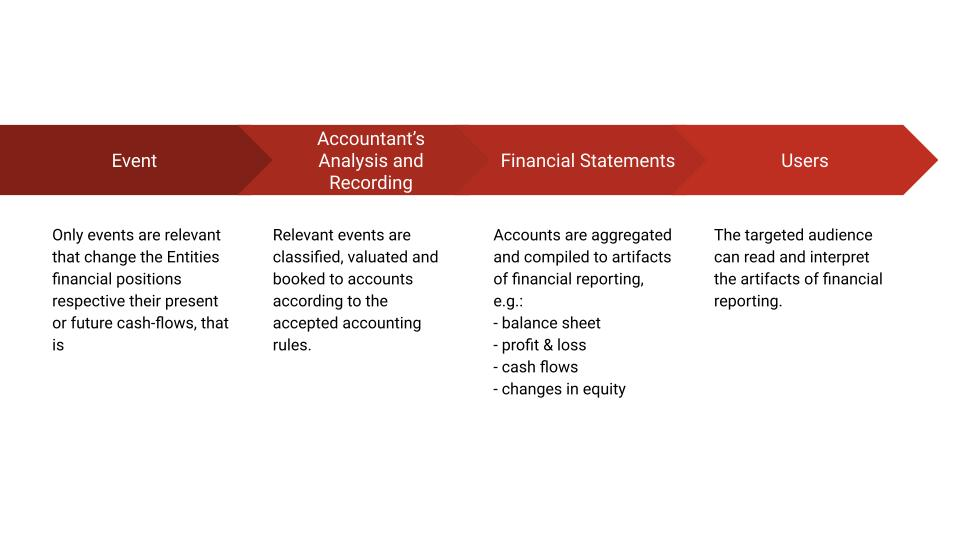
\includegraphics[width=0.7\textwidth]{../figures/Financial Accounting - fundamental relationships}
	\caption*{After \cite[p.3]{Horngren1984}: This figure indicates a process by setting general steps in an ordered relationship.} 
\end{figure}

The mentioned \enquote{accounting process} requires the identification of \enquote{transactions as they affect an organization}(\cite[p.13]{Horngren1984}).
Therefore \cite[p.13]{Horngren1984} introduces the entity as \enquote{specific area of accountability, a center of attention, a clear-cut boundary for reporting.}

The IASB Framework sets the entity as a reporting boundary:\cite[1.13]{IASBFramwork}

\blockquote{Information about the nature and amounts of a reporting entity’s economic resources and claims can help users to identify the reporting entity’s financial strengths and weaknesses. That information can help users to assess the reporting entity’s liquidity and solvency, its needs for additional financing and how successful it is likely to be in obtaining that financing. That information can also help users to assess management’s stewardship of the entity’s economic resources. Information about priorities and payment requirements of existing claims helps users to predict how future cash flows will be distributed among those with a claim against the reporting entity}

\cite{IASBFramwork} 

\blockcquote[3.4]{IASBFramwork}{Financial statements are prepared for a specified period of time (reporting period) and provide information about:
\begin{itemize}
	\item[] (a) assets and liabilities—including unrecognised assets and liabilities—
	and equity that existed at the end of the reporting period, or during
	the reporting period; and
	\item[] (b) income and expenses for the reporting period
\end{itemize}
}

\blockcquote[3.10]{IASBFramwork}{A reporting entity is an entity that is required, or chooses, to prepare financial statements. A reporting entity can be a single entity or a portion of an entity or can comprise more than one entity. A reporting entity is not necessarily a legal entity}

Imporatant is to distinguish between a company and its owner. In financial accounting, the company is the legal entity and therefore defines the point of view and the owner has rights on the companies assets.


% Usually a entity in this context is equivalent to a company.
Financial accounting always uses this boundary "what happens within my companies" but is never really reflecting other entities, besides 3rd parties in ageing lists.
Usually an entity represents a company and only this company.
Owners capital is reflected as equitiy and investments in other companies are usually subsumed as financial assets.
The entity acts therefore as point of view where only present and future financial transactions affecting the entity are in scope.
Both refer to the term \enquote{Entity} (also refer to as company, organization ) as subject, that sets the point of view and als the boundary for events relevant for Financial Accounting.
\todo{Insert Venn Diagram for Events: General Event, Business Event, Financial Event}

\subsection{Recognizable elements of financial statements}

\todo{Indicator for control over a resource: Present and future Cash flows as very important indicator }
Eingehen darauf, was wann erkannt wird: z.B. Fokus nicht nur auf Ereignisse das Unternehemn betreffend sondern ganz explizit mit direkten finanziellen Auswirkungen. (Einengen der Entity)
Weiter machen mit dem generellem Zeitpunkt des Erkennens

\todo{IASB 4.1 and 4.2 }

\todo{REcognition criteria IASB 5.6}

\todo{Horngren p. 13 - Transactions as exampel}


\begin{table}
	\caption{The elements of financial statements}\label{tab:elementsfinancialstatements}
	\begin{center}
% \begin{tabular}{|p{0.3\textwidth}|p{0.15\textwidth}|p{.5\textwidth}|}
	\begin{tabular}{|p{3,5cm}|p{2cm}|p{7,1cm}|}
	\hline
	Economic resource &
	  Asset &
	  A present economic resource controlled by the entity as a result of past events.
	  
	  An economic resource is a right that has the potential to produce economic benefits. \\ \hline
	Claim                                          & Liability & A present obligation of the entity to transfer an economic resource as a result of past events. \\ \cline{2-3} 
												   & Equity    & The residual interest in the assets of the entity after deducting all its liabilities           \\ \hline
	Changes in economic resources and claims, reflecting financial performance &
	  Income &
	  Increases in assets, or decreases in liabilities, that result in increases in equity, other than those relating to contributions from holders of equity claims. \\ \cline{2-3} 
	 &
	  Expense &
	  Decreases in asssets, or increases in liabilities, that result in decreases in equity, other than those relating to distributions to holders of equity claims. \\ \hline
	Ohter changes in economic resources and claims & -         & Contributions from holders of equity claims, and distributions to them.                         \\ \cline{2-3}
												   & -         & Exchanges of assets or liabilities that do not result in increases or decreases in equity.      \\ \hline
	\end{tabular}
	
\end{center}
	\caption*{This table from \cite[Section 4.2]{IASBFramwork} gives an overview of different elements that are recognized in financial statements.}
\end{table}








\section{Measurement and Valuation}


% \todo{IASB 5.4}


As mentioned in previous section \ref{sec:Finacc-Picture} accounting can be understood as "continuos, permanently changing picture" of an Entities resources.
To be able to "paint" this picture a process to 
Hier den Prozess skizzieren\dots




Financial accounting is often referred to as methodology to give an insight over the financial position of a company\dots
% \todo{Weiter ausarbeiten: Die Entity als Eventhorizont, Events als Auslöser von Veränderungen, Sichtweisen von Financial accounting (Moxter)}


In this chapter aspects of financial accounting most relevant for this thesis are introduced.
Most of interest are aspects that concern of a perspective of Accounting as a processing of events combined with the view from within a company as subject.
There are:k
\begin{itemize}
	\item Event recognition - are events relevant for entity.
	\item Event classification
	\item Event valuation
	\item 
\end{itemize}
\section{Profit \& Loss and the concept of accrual}
\section{Accounting Theories}

Although financial accounting and double entry accounting is known used since medieval formal standards barely existed until beginning of the 20th century.
Three different financial theories (dogmas) are summarized in \cite{moxter1984BilanzlehreI}, namely the 



Task: - find sufficient conecepts to map the REA data model to classical double entry book keeping.
-- use dynamische Bilanz for that purpose because:
-- Balance sheet entries are floating posts that are only temporary as soon as the business transaction is finished
-- Same IDEA for REA: A REA transaction is done, when all events for this transaction is done
-- At the end of the entity all floating items have to be resolved, if a company is shot down there never are unresolved items in a balance sheet. (and also not in the balance sheet at the start (except equity))


Moxter has three different Financial Accounting Theories

Moxter beschreibt in \cite{moxter1984BilanzlehreI} verschiedene Herangehensweisen.

Statische Bilanz => Ausgehend vom Vermögen
Dynamische Bilanz => Ausgehend von G\&
V (Siehe Beispiel einer kurzlebigen Unternehmung)



\section{Basic Picture of Accounting - Valuation \& Recognition Financial Accounting as process}





and introduces the concept of principals and surrogates to do a projection of real wordl predicates to a complete projection, that is all events that are relevant (for an entity) can be found in that view (in this case accounts).
Picture: Projection

Valuation by Rules Ijiri Page 94f.


The company in Financial Accounting is reflected as closed entity that has control over resources.
Measurment happens by events that change the control over resources.


While Financial Accounting is a stedy process of Recognition of 




\subsection{Three concepts}
Base for this projection is always the event horizon of an entity, I want to elaborate on three important concepts:

\subsection{Event horizon of the Entity}

\subsection{Resource and the axiom of control}

\subsection{Events that affect the resources under control}


\subsection{Process of Accounting}
Horngreen summarizes the process as follows, 

Measurement -> Brücke zu Ijiri

Classificational vs. Causal accounting


\section{Aspects of dynamic accounting in connection to REA}

Diese DA behandelt zwar "nur" die Buchhaltungstechnik, es scheint aber sinnvoll die Perspektive der dynamischen Bilanztheorie einzunehmen,
da "Ereignisse" in REA im weitesten Sinne eine Veränderung im Bestand verursachen und daran eine Analog gezogen werden kann.

%\item Dynamische Bilanz -> verschiedene Fälle







\section{The purpose of financial Accounting}
After Horngren, Accounting in general is the profession executed by Accountangs to \enquote{design their system after considering the types of information desired and other users}.\cite{Horngren1984}[p.3]
The desired informations are commonly used to answer questions after the perfomance of a \enquote{organization} in a given period and the (financial) standing in a certain moment in time.\cite{Horngren1984}[p.3]

\section{Artefacts in Financial Accounting}

\subsection{Debit and Credit}
=> Debit und Credit sind nur Begriffe 

Ijiry (as additional source) states that \enquote{Accounting is a system for communicating the economic events of an entity}. \cite{Ijiri1967}[p.3]
That is \enquote{The economic events of an entity must be represented by an organized set of symbols which are suitable for communication}. \cite{Ijiri1967}[p.3]

The most resulting artifacts of financial accounting activity are the income statement and the balance sheet.
\enquote{To obtain these statements}

\todo{Ijiri surrogates}




An event get's recognized, then it must be analyzed if it is relevant for financial position of the entity / if it changes the financial position of the entity.
Then Measurment, then classification

\section{Relevenace of Events }
An Event has to as to affect the financial position to be recognized in accounting 

For this to be true everey event has to analyzed for it's implicatoins

First it h of the entity
Secon it's classification 

realizatoin

Different types of events:
Business Event
Financial Event










\section{Causal accounting}

2021-09-12

This thesis considers two approaches to the basics of financial accounting.



+++++++

Excerpt: How can the consumption of services be modelled?

Intro: Horngren argues that every purchase of service as expense goes through balance sheet:
- Purchase on Assets for immediate consumption
- Consumption of service as expense
=> It is a kind of depreciation

In REA the first booking is easy:
Resource Money is exchanged against resource "Service".
But then this "Service" has to be consumed against what?

But: The benefit of "Service" stays inside the company, is it a kind of depreciation?
So this could be modeled as a pure financial event.

+++++++



The understaning of doing business and measuring the success has drastically changed over the past years.
Companies are required to deliver financial information at any time.
Thinking of Italian traders in the medieval age the motivation to account business transactions then today:
Back then it was usual to not have an annual closing, they rather calculated the success of a long lasting trade trips on a per trip base over years as Eugen Schmalenbach states:

\blockquote[\cite{schmalenbach1962}][]{Hier das Zitat!!!}

The trader did business on his own and a sum up was done after all related transactions where finished.
So there was no need to distungish between the owne and the company and also no need for accruals.

Schmalenbach starts with a hyphotetic business that lives only for a single purpose and is rolled up after this purpose is over.
The business gets credit from banks 
Within the lifetime of this company only incomes and expenses measured and at the end a single balance sheet is created:
All 
This balance sheetare aufgelöst after the purpose of this company i

Unterscheidung Aufwand und Ausgaben


Financial accounting took a long way from medeval ages where the economic success was calculated by economic long term project there was no difference between. Success was calculated after a cruise accross the ocean was finished on per project base, a yearly financial statement was unkown and not in focus.

Time after time and as money markets arised it was more and more important to give a complete view.


Following these requirements the P \& L oriented structured balance sheet 

A financial statement has to fullfill many requirments: It should give Investors an insight

Over time a company is considered as independent 










As kind of grounding of this thesis foundations of Accounting are investigated in this chapter.
The starting point is an overview over the process of accounting and fundamental terms of accounting, the main source for that part will be \cite{Horngren1984}.
Then fundamental connections between events, resources and following implications for measurment, classification and valuations are considered, this part will heavily rely on \cite{Ijiri1967}.
At last IFRS as concrete standard for measurement and classification is introspected as this will be the basis for mapping activities between the REA Data Model and financial accounting artefacts.
starting with the process of accounting, going further to typical artefactes and an analysis of mechanics in accounting.

The well known double entry accounting with it's first written introduction in \ldots by \ldots is widely anticiptated. % and worldwide used.
\enquote{Accounting is the major means of communicationg about the financial impact of an organzation's activities.}\cite[p.3]{Horngren1984}
It's
It's main artefacts are t-accounts, journals and as core the so called ALE Equation.

But what is behind the scenes?


To make rational choices, comprehensive information about a companies wealth to interested actors / audience is crucial.
Financial Accounting supports these decisions by delivering an overview over a companies assets and liabilities and Accrual Accounting extends this support by making the companies performance in a given period visible.

This chapter introduces fundamentals of Accounting and presents the audience and their benefits of the accrual accounting artefacts and relates fundamental concepts of accrual and further IFRS accounting to REA\textcopyright accounting.
% The outcome will be an answer, if the REA Accounting Model is feasable to 

Scope: Financial Accounting -> financial reporting: e.g. values of assets, cash, income-statement

Financial Reporting as statutary reporting

Historical: Accounts where closed when , there where 

We mean financial reporting as statutory reporting as it is needed to inform Owners, Creditors and tax authorities that has to be done at least once a year and structured as defined by laws or regularities

History of accounting\dots
Balance sheet was rather a Reume over projects (like sailings) rather than a regulary executed task.
Often a balance was taken when the main journal was full and a new book was startet.

Intention of balance sheet:
Overview over capital
Calculation of Earnings in a period
Schmalenbach calls this a dynamic balance, where in dopik the Profit \& Loss account is embeded between to balances.

Historicaly there was a lot of discussion about valuation of items, higher taxrates e.g. yield to a motiviation to minimize wealth and financial result to tax optimization.
The only intention of analysis financial accounting in this thesis is solely technical based.

There are different kind of events possible: once that are relevant for the business but not for finincial reporting, events that are relevant also for financial accounting and events that only exist to have propber visible accounting e.g. events that are deducting assets or to do the annual closing.



Start with cash -> then accrual


% \enumerate{}
Stake holders, why do we do accounting: Investors
Accounting terms: Entity, Transaction, Valuation, Measurement
Transaktion starts with events.
Events can be relevant for Business, or have a financial impact (beispiel ijiri manager)
Duration of events (ijiri?)

\section{The process of accounting}
Process of accounting: recognizing an event relevant for financial accounting, valuation

\begin{figure}
	\centering
	\caption{Process of Accounting}
	\label{fig:accounting-process}
	\includegraphics[width=0.7\linewidth]{"../figures/replace/CollaborativePerspective"}
	\caption*{Taken from \cite[p.3]{horngren2006introduction}. This figure }
\end{figure}


\section{Foundations of Accounting}
REA itself is an accounting model but let's recap what the most important
properties of accounting are. \todo{citation! to REA Paper}

These foundations of accounting provide the grounding for the following check of common properties and possibilities for wmapping.

\subsection{The Entity}
The entity represents the event horizon of an Financial Accounting System.
An Entity can be a company, a department or also a group of companies and an Financial Accounting system must be assigned to exactly one.
Everything that touches the financial positions of an corresponding (zugehörig) entity is recorded.
Everything else is ignored.\cite[p.15]{Horngren1984}

If an employee gets sick that possibly leads to damage (e.g. by delaying projects) to the entity but this event will not yet find it's way to a Financial Accounting System as he will be receiving is usual salaries.
For paid leaves there is a need to build a provision in case the employee leaves the entity and can not consume his quota.
So when he is going on holidays this will be reflected in Financial Accounting as the quota is reduced.

REA itself was also designed as entity centric accounting system but then extended to an \enquote{Open-edi Business Transaction Ontology (OeBTO)}\cite[Figure 2]{ISOIEC1594442015}\ref{fig:collaborative-perspective}.
Although the concepts of REA allow a wider view on Accounting systems in this thesis the \enquote{Trading Partner View} is used as there exists no collaborative spac in Financial Accounting Systems and to make the mapping between Financial Accounting and REA Accounting simpler and support better understanding.
As preview, it is preferable that events relevant for Financial Accounting are depicted either as \enquote{credit} or \enquote{debit} as shown in \cite{schwaiger2015aleandrea} and make sense only from the entity's point of view.

% \begin{figure}
% 	\centering
% 	\caption{REA Collaborative Perspective}
% 	\label{fig:collaborative-perspective}
% 	\includegraphics[width=0.7\linewidth]{"../figures/replace/CollaborativePerspective"}
% 	\caption*{Taken from \cite[Figure 2]{ISOIEC1594442015}. This figure demonstrates the two possible point of views that can be used. In this thesis the collaborative space is not relevant therefore the \enquote{Trading Partner View} is used.}
% \end{figure}

\subsection{Purpose of accounting}
Audiences
Scope of accounting: Support of Decisions, AUD IT GAAP => Tax
\subsection{Recognition of Events}

Accounting is generally speaking the process of recognizing relevant event, to analyse and store them and finally create financial statements that can be interpreted by interested audience.
What kind of events and when they are in scope of finance accounting is

Financial accounting stores only interpreted and aggregated data in monetary units whereas REA recognizes the events with all their attributes itself.
McCarthy calls this the \enquote{essence of events}\todo{citing}.
Figure \ref{fig:EventsTimeOfRecording} shows the process of accounting and compares the moment of recognition through in financial accounting and REA accounting in a timeline.
It must be considered, that not every
\begin{figure}
	\centering
	\caption{Time of recording in Accounting systems}
	\label{fig:EventsTimeOfRecording}
	\includegraphics[width=0.7\linewidth]{"../figures/EventsTimeOfRecording"}
	\caption*{This figure after \cite{Horngren1984} shows the different moments in time when recording happens. Traditional accounting first interprets the event and records the interpretation whereas REA stores all needed information of an event to interpret it afterwords.}
\end{figure}

\subsection{Management and Financial Accounting}
Purpose of accounting: Targeted Audience, difference between management and
financial accounting
\section{Concepts of Financial Accounting}
\subsection{The Statement of Financial positions}
The statement of financial positions is also called \enquote{balance sheet} as this equation has always to be true:
\[ Assets = Equities \]
The Assets consist of resources, that are under the equities control and the Equities can be further distinguished to:
\[ Equities = Liabilities + Shareholders equity\]


Different Types of Assets:

Tangible \& Intangible

Financial Assets

Direct tradable Assets acting as resources: Tangible \& intangible Assets,
Inventories, Cash

Discussion of Claims

Assets have nature of commitmens of other companies for future resource flow

Problem: Commitments can not be exchanged but this is possible with Assets that have only one borrower

\subsection{Liabilities}
Claim not feasable

Commitment

\subsection{The income statement}
Accrual accounting here\ldots

Development of equation

Debit / Credit

Changes in Equity\ldots

Different Types of bookings:
Even Services are in fact

=> Events that have effect to income statement and events that have not.

Accrual Accounting: Revenue and Expense are connected

2 Beispiele: Kauf von Verbrauchsmaterial => 1) Sofortige Abschreibung 2) Kauf auf Lager, dann Verkauf => Muss bei Mapping von Events berücksichtigt werden / Oder hängt es an der Resource? Lagerresource vs. Verbrauchsresource Inventoryresource vs. consumables

\section{Accrual Accounting}
Special ledgers: Creditors, Debitors, Ageing




\section{IFRS Accrual Accounting}
Usual artefacts out of IFRS Accounting: Balance Sheet, Income Statement, Changes in Equity, Cash Flow
Other usefull artefacts: Ageing list by business partner,


More or less interresting for valuation and recognition, not technical
modelling.

Will be used for Case study\ldots




\begin{table}
	\caption{}\label{tab:Elementary concepts}\caption*{}
	\begin{tabular}{|p{0.15\linewidth}|p{0.15\linewidth}|p{0.15\linewidth}|p{0.55\linewidth}|}
		\hline
		Categorie & Accrual Accounting & REA\textcopyright{} Accounting & Analysis result
		\\
		\hline
		Scope     & Entity             & REA Internal View              & REA itself can be used from an outside or
		inside entities viewpoint. In this thesis the internal viewpoint is
		choosen
		\\
	\end{tabular}
\end{table}

\section{Summary}
In this chapter the foundations of Financial Accounting and the resulting ALE Datamodel where presented.
The Event based character of Financial Accounting was studied and the process behind that leads to this Datamodel was analyzed.

It was pointed out, that conceptualy double entry accounting is a surrogate for real events, so every booking represents an event identified as relevant to an entities financial positions.

The \enquote{Double Entry Accounting} is a common notation for an \enquote{ALE Date Model} that technicaly stores these analyzed events on the \enquote{debit} or \enquote{credit} side of an Account so that the \enquote{ALE Equation} holds.
Nevertheless especially \enquote{debit} and \enquote{credit} don't hold any semantic meaning and are merely technical terms to acomplish this restriction and their interpretation depends on the class of the booked Account.

The dynamic nature of \enquote{Accrual Accounting} was explored and also the impact of past, present and future events.
Different Accounting Theories and their different views on Financial Accounting where outlined.

Also the difference between classificational and causal accounting was discussed, whereas in causal accounting every change in financial positions is connected to an event that causes that change.

With this knowledge about the mechanics behind Financial Accounting a mapping will be done in Chapter 3 \todo{Insert reference}.
% \input{Chapter03_REACFinancialAccountingModel}
% \input{Chapter04_CaseStudy}
% \input{Chapter05_SummaryConclusion} 
% \input{A_Chapter03_IFRSAccrualAccounting}
% \input{A_Chapter04_DesignOfCommitmentDuality}
% \input{Chapter03_REAInDeep}
% \input{Chapter04_DomainAccrualAccounting}
% \input{Chapter05_Mapping}
% \input{Chapter06_CaseStudy}
% \input{Chapter07_SummaryConclusion} 
%\appendix
% \input{ChapterXX_Appendix}

\backmatter

% Use an optional list of figures.
%\listoffigures % Starred version, i.e., \listoffigures*, removes the toc entry.

% Use an optional list of tables.
%\listoftables % Starred version, i.e., \listoftables*, removes the toc entry.

% Use an optional list of alogrithms.
%\listofalgorithms
%\addcontentsline{toc}{chapter}{List of Algorithms}

% Add an index.
%\printindex

% Add a glossary.
%\printglossaries

%Also include not-used bibtex entries
%\nocite{*}
% Add a bibliography.
\bibliographystyle{alpha}
\bibliography{../References/References}

\end{document}